\documentclass{article}
\usepackage[utf8]{inputenc}
\usepackage{float}
\usepackage{graphicx}
\usepackage{amsmath}

\title{dRegAut afl 2}
\author{Hanus Rindom}
\date{May 2014}

\begin{document}

\maketitle

\section{Intersection}
produktkonstruktionen af automat for sprogene $ L(M_1) \bigcap L(M_2) $.
\begin{figure}[h]
    \caption{Intersection}
        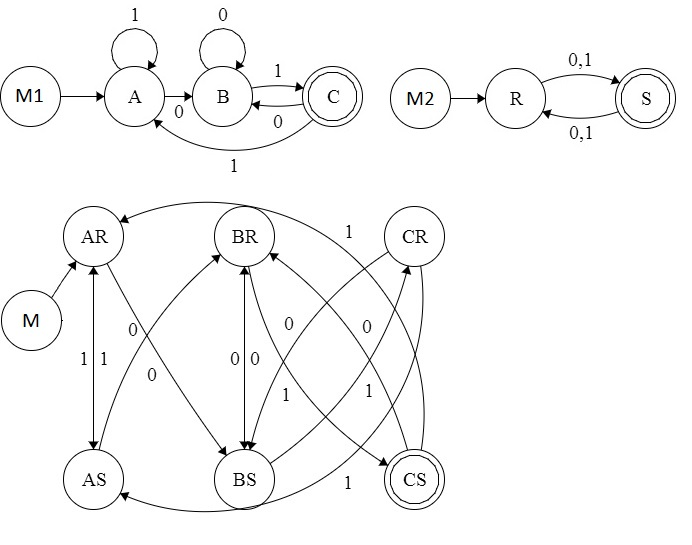
\includegraphics[width=1\textwidth]{download}
\end{figure}

\begin{figure}[h]
    \caption{Intersection, bedre opstillet}
        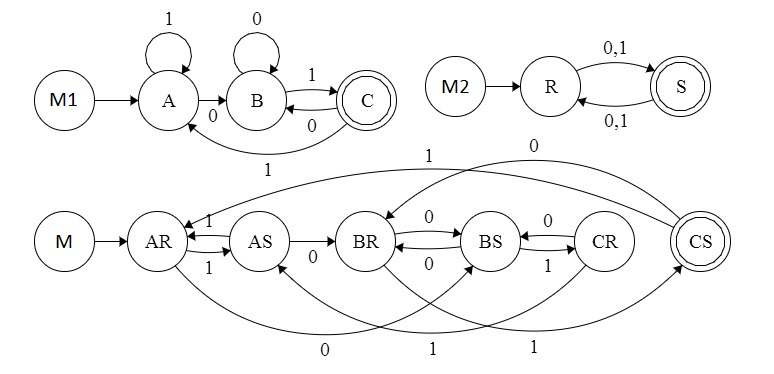
\includegraphics[width=1\textwidth]{download2}
\end{figure}
Konstruktureret ud fra Therom 2.15.\\
Vi får givet $ M_1 $ og $ M_2 $ og skal konstruere $ M $.\\
$$ L_1= \{ x \in \{ 0,1 \}* | \text{ x ender med 01} \} $$
$$ L_2= \{ x \in \{ 0,1 \}* | \text{ x er ulige} \} $$

M er den nye automat med tilstanden(e) $ Q=Q_1 \times Q_2 $ og starttilstanden $ q_0 = (q_1 , q_2) $\\

Alle transitionsfunktionerne gennemgås, hvilket kan illustreres med formlen:
$$ \delta((p,q), \sigma) = \delta _1 (p, \sigma), \delta _2 (q , \sigma) $$

For alle $ p \in Q_1 $, $ q \in Q_2 $ og $ \sigma \in \Sigma $ gælder accepttilstanden af sproget L:
$$ A= \{ x \in \{ 0,1 \}* | \text{ x ender med 01 og x er ulige} \} $$

\end{document}
